\documentclass[11pt,a4paper]{article}

\usepackage[utf8]{inputenc}
\usepackage[T1]{fontenc}
\usepackage{lmodern}
\usepackage[margin=2.2cm]{geometry}
\usepackage{xcolor}
\usepackage{listings}
\usepackage{booktabs}
\usepackage{array}
\usepackage{enumitem}
\usepackage{hyperref}
\usepackage{tikz}
\usetikzlibrary{arrows.meta,positioning,shapes.geometric,fit}

\definecolor{codebackground}{HTML}{F5F7FA}
\definecolor{codeborder}{HTML}{CBD5E1}
\definecolor{codegreen}{HTML}{166534}
\definecolor{codeblue}{HTML}{1D4ED8}
\definecolor{codeorange}{HTML}{C2410C}
\definecolor{codered}{HTML}{B91C1C}
\definecolor{darktext}{HTML}{172033}

\hypersetup{
    colorlinks=true,
    linkcolor=codeblue,
    urlcolor=codeblue,
    pdftitle={Using Docker PostgreSQL in STOCKLAB},
    pdfauthor={STOCKLAB Project Guide}
}

\lstdefinestyle{terminal}{
    backgroundcolor=\color{codebackground},
    basicstyle=\ttfamily\small,
    frame=single,
    rulecolor=\color{codeborder},
    breaklines=true,
    showstringspaces=false,
    columns=fullflexible,
    keepspaces=true,
    xleftmargin=0.4em,
    xrightmargin=0.4em
}

\lstdefinestyle{python}{
    style=terminal,
    language=Python,
    keywordstyle=\color{codeblue}\bfseries,
    commentstyle=\color{codegreen},
    stringstyle=\color{codeorange}
}

\lstdefinestyle{sql}{
    style=terminal,
    language=SQL,
    keywordstyle=\color{codeblue}\bfseries,
    commentstyle=\color{codegreen},
    stringstyle=\color{codeorange}
}

\newcommand{\projectroot}{\texttt{/home/ghuy/STOCKLAB}}
\newcommand{\filename}[1]{\texttt{\detokenize{#1}}}

\newenvironment{important}
  {\begin{quote}\color{codered}\textbf{Important:}\ }
  {\end{quote}}

\newenvironment{result}
  {\begin{quote}\color{codegreen}\textbf{Expected result:}\ }
  {\end{quote}}

\title{\textbf{Using Docker PostgreSQL in STOCKLAB}\\
\large An Illustrated, Project-Specific Guide}
\author{STOCKLAB}
\date{August 24, 2026}

\begin{document}

\maketitle

\begin{abstract}
This guide explains how PostgreSQL, Docker, and the Python ETL code work
together in the STOCKLAB project. It provides a complete first-time setup,
explicit examples, database diagrams, inspection commands, and troubleshooting
steps. All commands assume that the current directory is \projectroot.
\end{abstract}

\tableofcontents
\newpage

\section{The Main Idea}

Docker runs only the PostgreSQL database. The Python application runs on the
host computer and connects to the database through TCP port \texttt{5433}.

\begin{center}
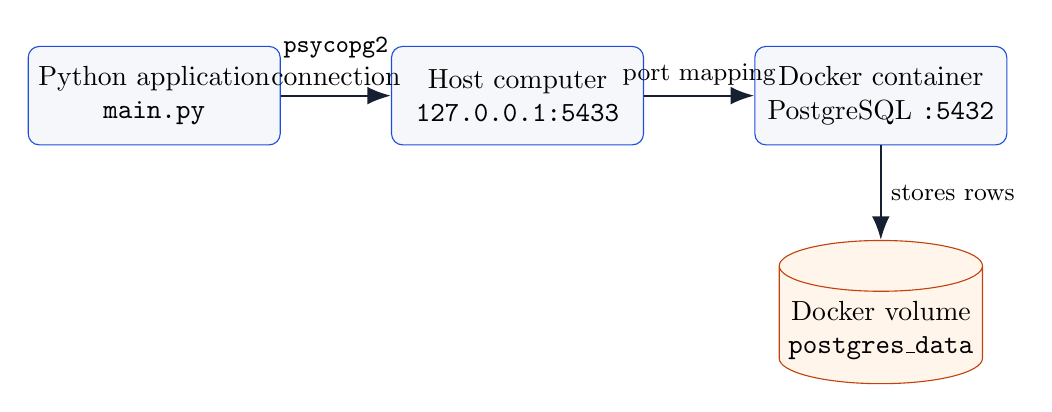
\begin{tikzpicture}[
    node distance=1.4cm,
    box/.style={
        draw=codeblue,
        rounded corners,
        align=center,
        minimum width=3.2cm,
        minimum height=1.25cm,
        fill=codebackground
    },
    store/.style={
        cylinder,
        shape border rotate=90,
        aspect=0.25,
        draw=codeorange,
        align=center,
        minimum width=2.5cm,
        minimum height=1.4cm,
        fill=orange!8
    },
    arrow/.style={-{Latex[length=3mm]}, thick, draw=darktext}
]
    \node[box] (python) {Python application\\
        \filename{main.py}};
    \node[box, right=of python] (hostport) {Host computer\\
        \texttt{127.0.0.1:5433}};
    \node[box, right=of hostport] (postgres) {Docker container\\
        PostgreSQL \texttt{:5432}};
    \node[store, below=1.2cm of postgres] (volume) {Docker volume\\
        \texttt{postgres\_data}};

    \draw[arrow] (python) -- node[above, align=center]
        {\small \texttt{psycopg2}\\connection} (hostport);
    \draw[arrow] (hostport) -- node[above]
        {\small port mapping} (postgres);
    \draw[arrow] (postgres) -- node[right]
        {\small stores rows} (volume);
\end{tikzpicture}
\end{center}

The mapping \texttt{5433:5432} means:

\begin{itemize}[leftmargin=2em]
    \item \texttt{5433} is the port used by programs running on your computer.
    \item \texttt{5432} is the PostgreSQL port inside the container.
\end{itemize}

\begin{important}
Because the Python program currently runs outside Docker, use
\texttt{DB\_HOST=127.0.0.1} and \texttt{DB\_PORT=5433}. Do not use the service
name \texttt{postgres} unless the Python application is later placed in another
Compose container.
\end{important}

\section{Current Project Configuration}

The project's \filename{docker-compose.yml} defines the following values:

\begin{center}
\begin{tabular}{>{\bfseries}p{4.3cm} p{7.7cm}}
\toprule
Setting & Current value and meaning \\
\midrule
Docker image & \texttt{postgres:17} \\
Container name & \texttt{vnstock-postgres} \\
Database & \texttt{vnstock} \\
Database user & \texttt{postgres} \\
Development password & \texttt{123456} \\
Host address & \texttt{127.0.0.1} \\
Host port & \texttt{5433} \\
Container port & \texttt{5432} \\
Persistent volume & \texttt{postgres\_data} \\
\bottomrule
\end{tabular}
\end{center}

The important part of the Compose file is:

\begin{lstlisting}[style=terminal]
services:
  postgres:
    image: postgres:17
    container_name: vnstock-postgres
    environment:
      POSTGRES_USER: postgres
      POSTGRES_PASSWORD: 123456
      POSTGRES_DB: vnstock
    ports:
      - "5433:5432"
    volumes:
      - postgres_data:/var/lib/postgresql/data
\end{lstlisting}

\section{First-Time Setup}

\subsection{Step 1: Open the project directory}

\begin{lstlisting}[style=terminal]
cd /home/ghuy/STOCKLAB
\end{lstlisting}

Run all remaining project commands from this directory. This is especially
important for the migration script because it opens
\filename{database/schema.sql} using a relative path.

\subsection{Step 2: Start PostgreSQL}

\begin{lstlisting}[style=terminal]
docker compose up -d postgres
\end{lstlisting}

The options mean:

\begin{itemize}[leftmargin=2em]
    \item \texttt{up}: create and start the service.
    \item \texttt{-d}: run it in the background.
    \item \texttt{postgres}: start only the PostgreSQL service.
\end{itemize}

Check its status:

\begin{lstlisting}[style=terminal]
docker compose ps
\end{lstlisting}

\begin{result}
The service should show a state such as \texttt{Up} or \texttt{running}, with a
port mapping similar to \texttt{0.0.0.0:5433->5432/tcp}.
\end{result}

If PostgreSQL is still initializing, follow its log:

\begin{lstlisting}[style=terminal]
docker compose logs -f postgres
\end{lstlisting}

Press \texttt{Ctrl+C} to stop following the log. This does not stop the
container.

\subsection{Step 3: Configure Python's database connection}

Create a file named \filename{.env} in the project root:

\begin{lstlisting}[style=terminal]
DB_HOST=127.0.0.1
DB_PORT=5433
DB_NAME=vnstock
DB_USER=postgres
DB_PASSWORD=123456
\end{lstlisting}

The file is read by \filename{database/connection.py}:

\begin{lstlisting}[style=python]
connection = psycopg2.connect(
    host=os.getenv("DB_HOST"),
    port=os.getenv("DB_PORT"),
    dbname=os.getenv("DB_NAME"),
    user=os.getenv("DB_USER"),
    password=os.getenv("DB_PASSWORD"),
)
\end{lstlisting}

\begin{important}
The password in \filename{.env} must match \texttt{POSTGRES\_PASSWORD} in
\filename{docker-compose.yml}. The current Python fallback password is empty,
so omitting \texttt{DB\_PASSWORD} will normally cause authentication to fail.
The project's \filename{.gitignore} excludes \filename{.env}; do not commit
real passwords.
\end{important}

\subsection{Step 4: Prepare the Python environment}

Create and activate a virtual environment:

\begin{lstlisting}[style=terminal]
python3 -m venv venv
source venv/bin/activate
\end{lstlisting}

Install the packages used by the database and ETL code:

\begin{lstlisting}[style=terminal]
python3 -m pip install psycopg2-binary python-dotenv pandas vnstock
\end{lstlisting}

Verify the PostgreSQL driver:

\begin{lstlisting}[style=terminal]
python3 -c "import psycopg2; print(psycopg2.__version__)"
\end{lstlisting}

\begin{result}
A version number is printed without a Python exception.
\end{result}

\subsection{Step 5: Create the tables}

The Compose service creates the \texttt{vnstock} database, but it does not
automatically create the STOCKLAB tables. Run:

\begin{lstlisting}[style=terminal]
python3 -m database.migrate
\end{lstlisting}

\begin{result}
The script prints \texttt{Database migrated successfully.}
\end{result}

It is safe to run the current migration again because the schema uses
\texttt{CREATE TABLE IF NOT EXISTS}.

\subsection{Step 6: Run the ETL application}

\begin{lstlisting}[style=terminal]
python3 main.py
\end{lstlisting}

The execution path is:

\begin{center}
\begin{tikzpicture}[
    node distance=0.85cm,
    step/.style={
        draw=codeblue,
        rounded corners,
        fill=blue!5,
        align=center,
        minimum width=8cm,
        minimum height=0.85cm
    },
    arrow/.style={-{Latex[length=2.5mm]}, thick}
]
    \node[step] (a) {\filename{main.py} loads \filename{stock_config.py}};
    \node[step, below=of a] (b) {The pipeline checks whether each symbol exists};
    \node[step, below=of b] (c) {Missing symbols are inserted into \texttt{stocks}};
    \node[step, below=of c] (d) {\texttt{vnstock} supplies historical prices};
    \node[step, below=of d] (e) {The data is cleaned and sorted};
    \node[step, below=of e] (f) {Rows are inserted into \texttt{daily\_prices}};

    \draw[arrow] (a) -- (b);
    \draw[arrow] (b) -- (c);
    \draw[arrow] (c) -- (d);
    \draw[arrow] (d) -- (e);
    \draw[arrow] (e) -- (f);
\end{tikzpicture}
\end{center}

The insert operations use \texttt{ON CONFLICT DO NOTHING}. Therefore,
re-running the pipeline does not insert a duplicate stock symbol or a duplicate
price for the same stock and trading date.

\section{Understanding the Database Schema}

\subsection{Entity relationship diagram}

\begin{center}
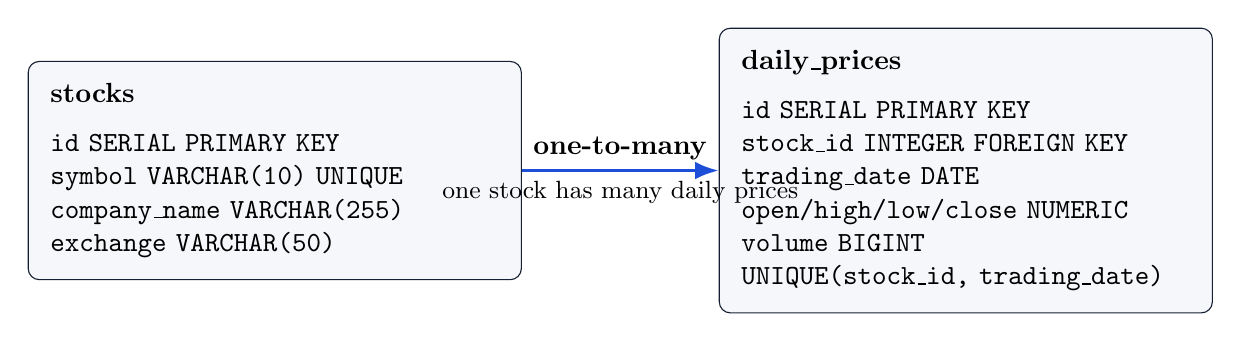
\begin{tikzpicture}[
    entity/.style={
        draw=darktext,
        rounded corners,
        align=left,
        text width=5.7cm,
        inner sep=8pt,
        fill=codebackground
    },
    relation/.style={-{Latex[length=3mm]}, very thick, draw=codeblue}
]
    \node[entity] (stocks) {
        \textbf{stocks}\\[2mm]
        \texttt{id SERIAL PRIMARY KEY}\\
        \texttt{symbol VARCHAR(10) UNIQUE}\\
        \texttt{company\_name VARCHAR(255)}\\
        \texttt{exchange VARCHAR(50)}
    };

    \node[entity, right=2.5cm of stocks] (prices) {
        \textbf{daily\_prices}\\[2mm]
        \texttt{id SERIAL PRIMARY KEY}\\
        \texttt{stock\_id INTEGER FOREIGN KEY}\\
        \texttt{trading\_date DATE}\\
        \texttt{open/high/low/close NUMERIC}\\
        \texttt{volume BIGINT}\\
        \texttt{UNIQUE(stock\_id, trading\_date)}
    };

    \draw[relation] (stocks) -- node[above]{\textbf{one-to-many}}
        node[below]{\small one stock has many daily prices} (prices);
\end{tikzpicture}
\end{center}

For example, the stock \texttt{FPT} appears once in \texttt{stocks}, while
each trading day for FPT is a separate row in \texttt{daily\_prices}.

\subsection{Concrete example}

Suppose the \texttt{stocks} table contains:

\begin{center}
\begin{tabular}{rlll}
\toprule
\textbf{id} & \textbf{symbol} & \textbf{company\_name} & \textbf{exchange} \\
\midrule
1 & FPT & FPT Corporation & HOSE \\
2 & VNM & Vinamilk & HOSE \\
\bottomrule
\end{tabular}
\end{center}

Then \texttt{daily\_prices} can contain:

\begin{center}
\small
\begin{tabular}{rrlrrrrr}
\toprule
\textbf{id} & \textbf{stock\_id} & \textbf{date} &
\textbf{open} & \textbf{high} & \textbf{low} & \textbf{close} &
\textbf{volume} \\
\midrule
1 & 1 & 2026-08-20 & 100.00 & 103.00 & 99.50 & 102.00 & 1200000 \\
2 & 1 & 2026-08-21 & 102.00 & 104.00 & 101.00 & 103.50 & 950000 \\
3 & 2 & 2026-08-21 & 65.00 & 66.00 & 64.50 & 65.50 & 710000 \\
\bottomrule
\end{tabular}
\end{center}

Rows 1 and 2 belong to FPT because their \texttt{stock\_id} is 1.

\section{Working Directly with PostgreSQL}

\subsection{Open the PostgreSQL shell}

\begin{lstlisting}[style=terminal]
docker compose exec postgres psql -U postgres -d vnstock
\end{lstlisting}

Your prompt should change to something similar to:

\begin{lstlisting}[style=terminal]
vnstock=#
\end{lstlisting}

\subsection{Useful \texttt{psql} commands}

\begin{lstlisting}[style=terminal]
\dt                         -- list tables
\d stocks                   -- describe the stocks table
\d daily_prices             -- describe the prices table
\l                          -- list databases
\q                          -- exit psql
\end{lstlisting}

Commands beginning with a backslash are \texttt{psql} commands, not SQL
statements, so they do not require a semicolon.

\subsection{Useful SQL queries}

Count stocks:

\begin{lstlisting}[style=sql]
SELECT COUNT(*) FROM stocks;
\end{lstlisting}

Display ten stocks:

\begin{lstlisting}[style=sql]
SELECT id, symbol, company_name, exchange
FROM stocks
ORDER BY symbol
LIMIT 10;
\end{lstlisting}

Count price rows for each stock:

\begin{lstlisting}[style=sql]
SELECT
    s.symbol,
    COUNT(dp.id) AS price_rows
FROM stocks AS s
LEFT JOIN daily_prices AS dp ON dp.stock_id = s.id
GROUP BY s.id, s.symbol
ORDER BY price_rows DESC;
\end{lstlisting}

Get FPT's latest ten prices:

\begin{lstlisting}[style=sql]
SELECT
    s.symbol,
    dp.trading_date,
    dp.open_price,
    dp.high,
    dp.low,
    dp.close_price,
    dp.volume
FROM daily_prices AS dp
JOIN stocks AS s ON s.id = dp.stock_id
WHERE s.symbol = 'FPT'
ORDER BY dp.trading_date DESC
LIMIT 10;
\end{lstlisting}

\subsection{Manual insert example}

Insert a sample stock:

\begin{lstlisting}[style=sql]
INSERT INTO stocks (symbol, company_name, exchange)
VALUES ('TEST', 'Example Company', 'DEMO')
ON CONFLICT (symbol) DO NOTHING;
\end{lstlisting}

Insert a sample price by looking up the stock ID:

\begin{lstlisting}[style=sql]
INSERT INTO daily_prices (
    stock_id,
    trading_date,
    open_price,
    high,
    low,
    close_price,
    volume
)
SELECT
    id,
    DATE '2026-08-24',
    10.00,
    11.00,
    9.50,
    10.50,
    100000
FROM stocks
WHERE symbol = 'TEST'
ON CONFLICT (stock_id, trading_date) DO NOTHING;
\end{lstlisting}

Verify the result:

\begin{lstlisting}[style=sql]
SELECT s.symbol, dp.*
FROM daily_prices AS dp
JOIN stocks AS s ON s.id = dp.stock_id
WHERE s.symbol = 'TEST';
\end{lstlisting}

Delete the demonstration data:

\begin{lstlisting}[style=sql]
DELETE FROM daily_prices
WHERE stock_id = (SELECT id FROM stocks WHERE symbol = 'TEST');

DELETE FROM stocks WHERE symbol = 'TEST';
\end{lstlisting}

\section{Using the Database from Python}

\subsection{Test the connection}

With the virtual environment active, run:

\begin{lstlisting}[style=terminal]
python3 -c "from database.connection import getConnection; \
c=getConnection(); print(c.get_dsn_parameters()); c.close()"
\end{lstlisting}

\begin{result}
Python prints connection parameters containing database
\texttt{vnstock}, host \texttt{127.0.0.1}, and port \texttt{5433}.
\end{result}

\subsection{Repository example}

The existing repository classes hide most SQL details:

\begin{lstlisting}[style=python]
from database.repository_stock import RepoStock
from database.repository_price import RepoPrice

stocks = RepoStock()
prices = RepoPrice()

print("Number of stocks:", stocks.count_stock())
print("FPT record:", stocks.get_stock("FPT"))
print(prices.get_price_limit("FPT", 5))
\end{lstlisting}

You can save this temporarily as a test script or run it in an interactive
Python session.

\subsection{Why parameterized queries matter}

The repositories correctly send values separately from the SQL:

\begin{lstlisting}[style=python]
sql = "SELECT id FROM stocks WHERE symbol = %s"
cursor.execute(sql, (symbol,))
\end{lstlisting}

Do not build the query with string concatenation. Parameterized queries handle
quoting correctly and protect the application from SQL injection.

\section{Preparing Price Data for a Correlation Matrix}

The correlation calculation needs one table in which:

\begin{itemize}[leftmargin=2em]
    \item each row represents one shared trading date;
    \item each column represents one stock symbol;
    \item each cell contains that symbol's closing price on that date.
\end{itemize}

The preparation process is:

\begin{center}
\begin{tikzpicture}[
    node distance=0.65cm,
    step/.style={
        draw=codeblue,
        rounded corners,
        fill=blue!5,
        align=center,
        minimum width=9cm,
        minimum height=0.75cm
    },
    arrow/.style={-{Latex[length=2.5mm]}, thick}
]
    \node[step] (a) {Read one symbol's rows from PostgreSQL};
    \node[step, below=of a] (b)
        {Keep \texttt{trading\_date} and \texttt{close\_price}};
    \node[step, below=of b] (c)
        {Convert the result into a date-indexed pandas Series};
    \node[step, below=of c] (d)
        {Append the Series to \texttt{price\_columns}};
    \node[step, below=of d] (e)
        {Use \texttt{pd.concat()} to combine all symbols};

    \draw[arrow] (a) -- (b);
    \draw[arrow] (b) -- (c);
    \draw[arrow] (c) -- (d);
    \draw[arrow] (d) -- (e);
\end{tikzpicture}
\end{center}

\subsection{The \texttt{prices} variable and its parentheses}

In the following code, \texttt{prices} is a variable. It is not a function:

\begin{lstlisting}[style=python]
prices = (
    df[["trading_date", "close_price"]]
    .dropna()
    .sort_values("trading_date")
)
\end{lstlisting}

The surrounding parentheses only allow a long Python expression to continue
across multiple lines. The same statement could be written on one line:

\begin{lstlisting}[style=python]
prices = df[["trading_date", "close_price"]].dropna().sort_values("trading_date")
\end{lstlisting}

Using multiple lines makes each transformation easier to read. A more explicit
variable name would be \texttt{symbol\_prices}, because the value represents
the prices for one symbol during one iteration of the loop.

\subsection{Selecting columns with double brackets}

The repository returns a DataFrame similar to:

\begin{lstlisting}[style=terminal]
  trading_date  open_price  high   low  close_price  volume
0   2026-08-20       100.0   105  99.0        103.0    5000
1   2026-08-21       103.0   107 102.0        106.0    6000
\end{lstlisting}

Correlation does not require the open, high, low, or volume columns. This
expression selects only the date and closing price:

\begin{lstlisting}[style=python]
df[["trading_date", "close_price"]]
\end{lstlisting}

The result is:

\begin{lstlisting}[style=terminal]
  trading_date  close_price
0   2026-08-20        103.0
1   2026-08-21        106.0
\end{lstlisting}

There are two pairs of brackets because they have different jobs:

\begin{enumerate}[leftmargin=2em]
    \item The inner brackets create a Python list of column names:
\begin{lstlisting}[style=python]
["trading_date", "close_price"]
\end{lstlisting}
    \item The outer brackets ask the DataFrame to select every column named in
    that list:
\begin{lstlisting}[style=python]
df[["trading_date", "close_price"]]
\end{lstlisting}
\end{enumerate}

Selecting one column uses a string and returns a pandas Series:

\begin{lstlisting}[style=python]
df["close_price"]
\end{lstlisting}

Selecting multiple columns uses a list and returns another DataFrame:

\begin{lstlisting}[style=python]
df[["trading_date", "close_price"]]
\end{lstlisting}

\begin{important}
The actual database column names in STOCKLAB are
\texttt{trading\_date} and \texttt{close\_price}. Names such as
\texttt{date} and \texttt{close} are not the column names returned by
\texttt{RepoPrice.get\_price\_all()}.
\end{important}

\subsection{Converting one symbol into a Series}

This transformation prepares one stock symbol:

\begin{lstlisting}[style=python]
symbol_prices = (
    df[["trading_date", "close_price"]]
    .dropna()
    .drop_duplicates(subset="trading_date", keep="last")
    .sort_values("trading_date")
    .set_index("trading_date")["close_price"]
    .astype(float)
    .rename(symbol)
)
\end{lstlisting}

Each operation has one purpose:

\begin{center}
\begin{tabular}{p{5.8cm} p{7.3cm}}
\toprule
\textbf{Operation} & \textbf{Purpose} \\
\midrule
\texttt{dropna()}
    & Remove rows whose selected date or closing price is missing. \\[1mm]
\texttt{drop\_duplicates(...)}
    & Keep only one row for each trading date. \\[1mm]
\texttt{sort\_values("trading\_date")}
    & Put the dates in chronological order. \\[1mm]
\texttt{set\_index("trading\_date")}
    & Use trading dates as row labels so pandas can align symbols by date. \\[1mm]
\texttt{["close\_price"]}
    & Select the closing-price column and produce a Series. \\[1mm]
\texttt{astype(float)}
    & Ensure the prices are numeric values suitable for NumPy calculations. \\[1mm]
\texttt{rename(symbol)}
    & Give the Series a name such as \texttt{VIC}, \texttt{VCB}, or
      \texttt{FPT}. \\
\bottomrule
\end{tabular}
\end{center}

For \texttt{symbol = "VIC"}, the result looks like:

\begin{lstlisting}[style=terminal]
trading_date
2026-08-20    103.0
2026-08-21    106.0
Name: VIC
\end{lstlisting}

The dates are now the Series index. This is important because pandas uses the
index to match the same date across different symbols.

\subsection{Why \texttt{price\_columns.append(symbol\_prices)} is needed}

The program processes one symbol at a time:

\begin{lstlisting}[style=python]
price_columns = []

for symbol in symbols:
    df = rpp.get_price_all(symbol)

    symbol_prices = (
        df[["trading_date", "close_price"]]
        .set_index("trading_date")["close_price"]
        .rename(symbol)
    )

    price_columns.append(symbol_prices)
\end{lstlisting}

\texttt{price\_columns = []} creates an empty Python list.
\texttt{append()} places one new item at the end of that list. For example:

\begin{lstlisting}[style=python]
numbers = []

numbers.append(10)
numbers.append(20)
numbers.append(30)

print(numbers)
\end{lstlisting}

The result is:

\begin{lstlisting}[style=terminal]
[10, 20, 30]
\end{lstlisting}

The correlation loop uses the same idea, but the items are pandas Series
rather than numbers. If:

\begin{lstlisting}[style=python]
symbols = ["VIC", "VCB", "FPT"]
\end{lstlisting}

then the list grows conceptually as follows:

\begin{lstlisting}[style=terminal]
After VIC:  [VIC_prices]
After VCB:  [VIC_prices, VCB_prices]
After FPT:  [VIC_prices, VCB_prices, FPT_prices]
\end{lstlisting}

The list temporarily collects every symbol's Series. After the loop finishes,
all of them can be combined in one operation.

\subsection{Combining symbols with \texttt{pd.concat()}}

Suppose the list contains three date-indexed Series:

\begin{lstlisting}[style=terminal]
VIC                     VCB                     FPT
2026-08-20  103.0       2026-08-20  65.0        2026-08-20  120.0
2026-08-21  106.0       2026-08-21  67.0        2026-08-21  123.0
2026-08-22  105.0       2026-08-22  66.0        2026-08-22  125.0
\end{lstlisting}

The following code combines them:

\begin{lstlisting}[style=python]
close_prices = pd.concat(
    price_columns,
    axis=1,
    join="inner"
).sort_index()
\end{lstlisting}

The resulting DataFrame is:

\begin{lstlisting}[style=terminal]
                VIC   VCB    FPT
trading_date
2026-08-20    103.0  65.0  120.0
2026-08-21    106.0  67.0  123.0
2026-08-22    105.0  66.0  125.0
\end{lstlisting}

\texttt{axis=1} means that pandas should combine the Series horizontally as
new columns. By comparison, \texttt{axis=0} would stack values vertically as
additional rows.

\texttt{join="inner"} means that pandas keeps only dates present in every
Series. For example, suppose VIC has prices for August 20, 21, and 22, but VCB
has prices only for August 20 and 22. The combined table is:

\begin{lstlisting}[style=terminal]
                VIC   VCB
trading_date
2026-08-20    103.0  65.0
2026-08-22    105.0  66.0
\end{lstlisting}

August 21 is excluded because VCB does not have an observation for that date.
This prevents the program from accidentally comparing returns from different
trading dates.

\subsection{Complete preparation example}

The complete data-preparation part can therefore be read in plain English as:
``fetch each stock, keep its date and close, save it in a list, and combine all
stocks by their shared dates.''

\begin{lstlisting}[style=python]
price_columns = []

for symbol in symbols:
    df = rpp.get_price_all(symbol)

    symbol_prices = (
        df[["trading_date", "close_price"]]
        .dropna()
        .drop_duplicates(subset="trading_date", keep="last")
        .sort_values("trading_date")
        .set_index("trading_date")["close_price"]
        .astype(float)
        .rename(symbol)
    )

    price_columns.append(symbol_prices)

close_prices = pd.concat(
    price_columns,
    axis=1,
    join="inner"
).sort_index()
\end{lstlisting}

Once \texttt{close\_prices} has this shape, log returns and their Pearson
correlation matrix can be calculated:

\begin{lstlisting}[style=python]
log_returns = np.log(
    close_prices / close_prices.shift(1)
) * 100

correlation_matrix = log_returns.dropna().corr(method="pearson")
\end{lstlisting}

\section{Daily Commands}

\begin{center}
\begin{tabular}{p{6.1cm} p{7.2cm}}
\toprule
\textbf{Command} & \textbf{Purpose} \\
\midrule
\texttt{docker compose up -d postgres}
    & Start or create PostgreSQL in the background. \\[1mm]
\texttt{docker compose ps}
    & Show the current container state. \\[1mm]
\texttt{docker compose logs -f postgres}
    & Follow PostgreSQL logs. \\[1mm]
\texttt{python3 -m database.migrate}
    & Create tables from \filename{schema.sql}. \\[1mm]
\texttt{python3 main.py}
    & Run the stock ETL pipeline. \\[1mm]
\texttt{docker compose exec postgres psql -U postgres -d vnstock}
    & Open the SQL shell. \\[1mm]
\texttt{docker compose stop}
    & Stop containers while keeping them and their data. \\[1mm]
\texttt{docker compose down}
    & Remove containers and network, but preserve the named volume. \\[1mm]
\texttt{docker compose down -v}
    & Remove containers and permanently delete the database volume. \\
\bottomrule
\end{tabular}
\end{center}

\section{Data Persistence}

PostgreSQL writes data to the named Docker volume rather than to the temporary
container filesystem.

\begin{center}
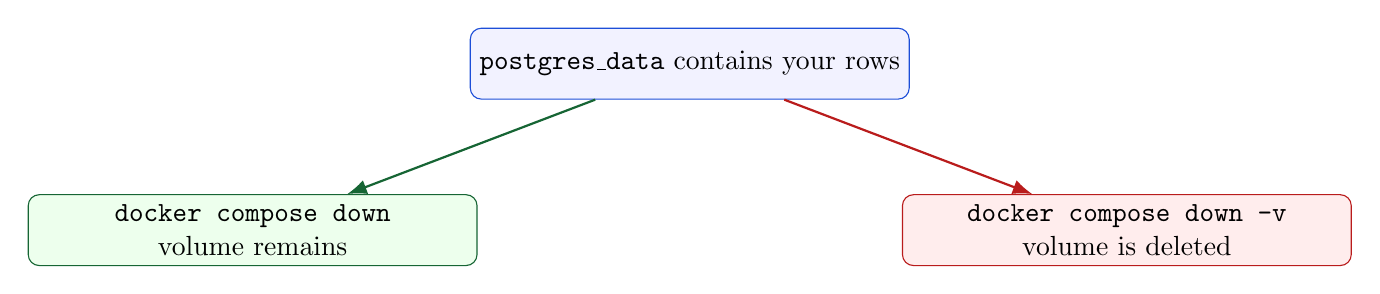
\begin{tikzpicture}[
    node distance=1.1cm,
    action/.style={
        draw=codeblue,
        rounded corners,
        fill=blue!5,
        minimum width=4.6cm,
        minimum height=0.9cm,
        align=center
    },
    safe/.style={
        draw=codegreen,
        rounded corners,
        fill=green!7,
        minimum width=5.7cm,
        minimum height=0.9cm,
        align=center
    },
    danger/.style={
        draw=codered,
        rounded corners,
        fill=red!7,
        minimum width=5.7cm,
        minimum height=0.9cm,
        align=center
    },
    arrow/.style={-{Latex[length=2.5mm]}, thick}
]
    \node[action] (volume) {\texttt{postgres\_data} contains your rows};
    \node[safe, below left=1.2cm and -0.1cm of volume] (down)
        {\texttt{docker compose down}\\volume remains};
    \node[danger, below right=1.2cm and -0.1cm of volume] (downv)
        {\texttt{docker compose down -v}\\volume is deleted};

    \draw[arrow, draw=codegreen] (volume) -- (down);
    \draw[arrow, draw=codered] (volume) -- (downv);
\end{tikzpicture}
\end{center}

\begin{important}
Use \texttt{docker compose down -v} only when you intentionally want a clean,
empty database. Afterward, start PostgreSQL again and rerun the migration.
\end{important}

\section{Troubleshooting}

\subsection{Quick diagnosis flow}

\begin{center}
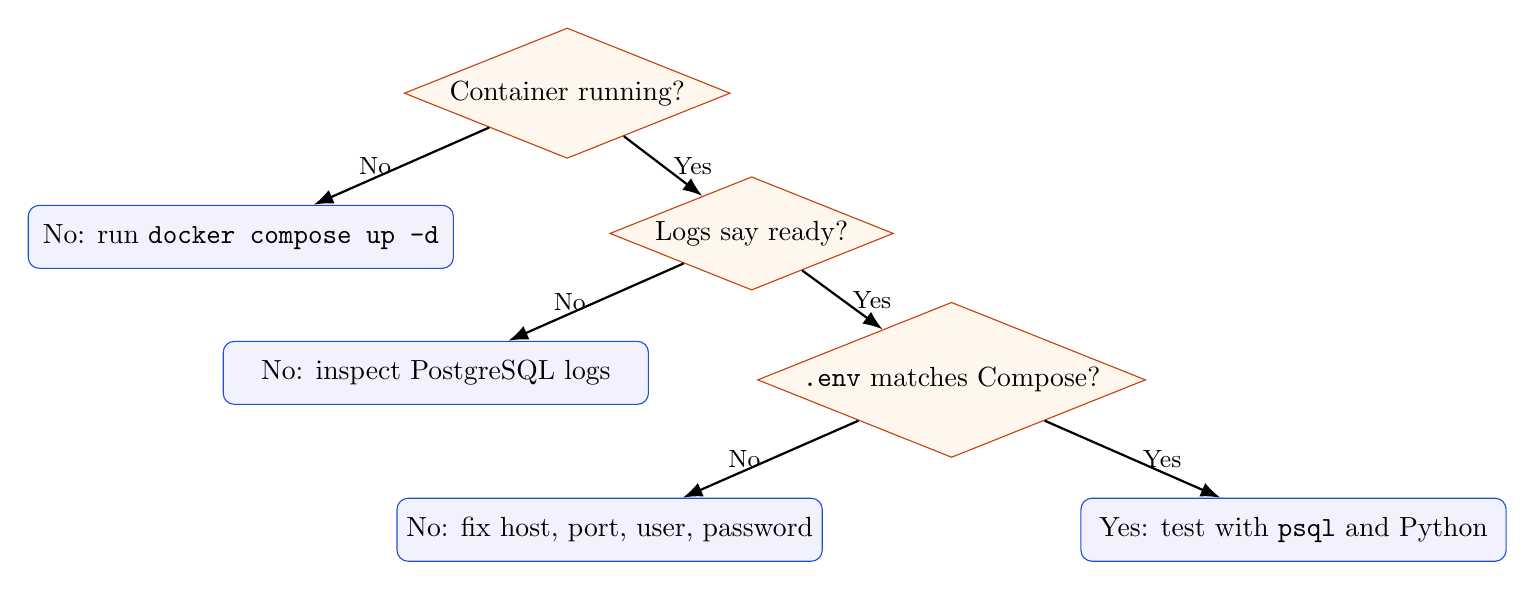
\begin{tikzpicture}[
    node distance=0.8cm,
    question/.style={
        diamond,
        draw=codeorange,
        fill=orange!7,
        aspect=2.5,
        align=center,
        inner sep=1.5pt
    },
    answer/.style={
        rectangle,
        rounded corners,
        draw=codeblue,
        fill=blue!5,
        align=center,
        minimum width=5.4cm,
        minimum height=0.8cm
    },
    arrow/.style={-{Latex[length=2.5mm]}, thick}
]
    \node[question] (running) {Container running?};
    \node[answer, below left=1cm and 0.4cm of running] (start)
        {No: run \texttt{docker compose up -d}};
    \node[question, below right=1cm and 0.4cm of running] (ready)
        {Logs say ready?};
    \node[answer, below left=1cm and 0.4cm of ready] (logs)
        {No: inspect PostgreSQL logs};
    \node[question, below right=1cm and 0.4cm of ready] (env)
        {\filename{.env} matches Compose?};
    \node[answer, below left=1cm and 0.4cm of env] (fixenv)
        {No: fix host, port, user, password};
    \node[answer, below right=1cm and 0.4cm of env] (test)
        {Yes: test with \texttt{psql} and Python};

    \draw[arrow] (running) -- node[left]{\small No} (start);
    \draw[arrow] (running) -- node[right]{\small Yes} (ready);
    \draw[arrow] (ready) -- node[left]{\small No} (logs);
    \draw[arrow] (ready) -- node[right]{\small Yes} (env);
    \draw[arrow] (env) -- node[left]{\small No} (fixenv);
    \draw[arrow] (env) -- node[right]{\small Yes} (test);
\end{tikzpicture}
\end{center}

\subsection{\texttt{permission denied} for \texttt{docker.sock}}

The command:

\begin{lstlisting}[style=terminal]
docker compose up -d
\end{lstlisting}

may return an error similar to:

\begin{lstlisting}[style=terminal]
unable to get image 'postgres:17': permission denied while trying
to connect to the Docker API at unix:///var/run/docker.sock
\end{lstlisting}

This message does not mean that the \texttt{postgres:17} image is unavailable.
Docker has not attempted to download the image yet. It means that the Docker
command-line program cannot access the Docker daemon through the Unix socket
\filename{/var/run/docker.sock}.

A common cause is that the user was added to the \texttt{docker} group after
the current terminal session was opened. The account's saved group membership
then includes \texttt{docker}, but the current shell has not loaded that
membership.

Check both the account configuration and the groups active in the current
shell:

\begin{lstlisting}[style=terminal]
id -nG
getent group docker
ls -l /var/run/docker.sock
\end{lstlisting}

The output from \texttt{id -nG} should include \texttt{docker}. The socket
normally has owner \texttt{root}, group \texttt{docker}, and permissions
\texttt{srw-rw----}.

If \texttt{getent group docker} lists your username but \texttt{id -nG} does
not list \texttt{docker}, activate the new group in the current terminal:

\begin{lstlisting}[style=terminal]
newgrp docker
id -nG
docker info
docker compose up -d
\end{lstlisting}

\texttt{newgrp docker} opens a new shell. The second command should now list
\texttt{docker}, and \texttt{docker info} should display information about
both the Docker client and server without a permission error.

Alternatively, close all terminals, sign out of the Linux desktop, and sign
back in. Merely opening another terminal may not be sufficient when the
desktop login session still has the old group list.

If the account is not yet a member of the Docker group, add it and then refresh
the login session:

\begin{lstlisting}[style=terminal]
sudo usermod -aG docker "$USER"
newgrp docker
docker info
\end{lstlisting}

If the problem remains, check the Docker service and repair unexpected socket
ownership:

\begin{lstlisting}[style=terminal]
sudo systemctl restart docker
sudo chown root:docker /var/run/docker.sock
sudo chmod 660 /var/run/docker.sock

docker info
docker compose up -d
\end{lstlisting}

\begin{important}
Do not use \texttt{chmod 666 /var/run/docker.sock}. Access to the Docker daemon
is effectively administrator-level access, so making the socket writable by
every local user creates a serious security risk.
\end{important}

If \texttt{systemctl} reports that the system was not booted with
\texttt{systemd}, the command may be running inside a development container
instead of the host operating system. Run Docker Compose from the host terminal
or configure the development container to receive the host Docker socket and
the socket's group ID.

\subsection{Password authentication failed}

Confirm that these values match:

\begin{itemize}[leftmargin=2em]
    \item \texttt{POSTGRES\_PASSWORD} in \filename{docker-compose.yml}
    \item \texttt{DB\_PASSWORD} in \filename{.env}
\end{itemize}

Changing \texttt{POSTGRES\_PASSWORD} after the database volume has already been
initialized does not automatically change the existing PostgreSQL user's
password. For disposable development data, reset the volume:

\begin{lstlisting}[style=terminal]
docker compose down -v
docker compose up -d postgres
python3 -m database.migrate
\end{lstlisting}

\begin{important}
The reset command deletes all existing database data.
\end{important}

\subsection{Connection refused on port 5433}

Check:

\begin{lstlisting}[style=terminal]
docker compose ps
docker compose logs postgres
\end{lstlisting}

Also verify that \filename{.env} contains:

\begin{lstlisting}[style=terminal]
DB_HOST=127.0.0.1
DB_PORT=5433
\end{lstlisting}

\subsection{Port 5433 is already in use}

Find the process using the port:

\begin{lstlisting}[style=terminal]
ss -ltnp | grep 5433
\end{lstlisting}

You can change the host side of the Compose mapping, for example:

\begin{lstlisting}[style=terminal]
ports:
  - "5434:5432"
\end{lstlisting}

Then also change \filename{.env}:

\begin{lstlisting}[style=terminal]
DB_PORT=5434
\end{lstlisting}

\subsection{\texttt{ModuleNotFoundError: No module named psycopg2}}

Activate the project's virtual environment and install the driver:

\begin{lstlisting}[style=terminal]
source venv/bin/activate
python3 -m pip install psycopg2-binary
\end{lstlisting}

\subsection{\texttt{relation "stocks" does not exist}}

The database is running, but the schema has not been applied:

\begin{lstlisting}[style=terminal]
python3 -m database.migrate
\end{lstlisting}

\subsection{The database is running but the ETL has no rows}

Separate database problems from API or transformation problems:

\begin{enumerate}[leftmargin=2em]
    \item Confirm the tables exist with \texttt{\textbackslash dt}.
    \item Run \texttt{SELECT COUNT(*) FROM stocks;}.
    \item Read the Python terminal output for rate-limit or extraction errors.
    \item Test one repository query from Python.
    \item Check \filename{stock_config.py} for symbols and ETL mode.
\end{enumerate}

\section{Development Security Notes}

The password \texttt{123456} is acceptable only as an isolated local
development example. For shared machines, deployed systems, or remotely
accessible databases:

\begin{itemize}[leftmargin=2em]
    \item use a long random password;
    \item do not hard-code secrets in a committed Compose file;
    \item keep secrets in an uncommitted environment file or secret manager;
    \item do not expose PostgreSQL to the public internet;
    \item create an application user instead of using the PostgreSQL
          administrator account.
\end{itemize}

\section{Complete Start-to-Finish Example}

The following sequence represents a clean first run:

\begin{lstlisting}[style=terminal]
cd /home/ghuy/STOCKLAB

docker compose up -d postgres
docker compose ps

python3 -m venv venv
source venv/bin/activate
python3 -m pip install psycopg2-binary python-dotenv pandas vnstock

# Create .env in the project root with the values from this guide.

python3 -m database.migrate

docker compose exec postgres \
  psql -U postgres -d vnstock -c "\dt"

python3 main.py

docker compose exec postgres \
  psql -U postgres -d vnstock \
  -c "SELECT COUNT(*) AS stocks FROM stocks;"

docker compose exec postgres \
  psql -U postgres -d vnstock \
  -c "SELECT COUNT(*) AS prices FROM daily_prices;"
\end{lstlisting}

For later sessions, the shorter normal workflow is:

\begin{lstlisting}[style=terminal]
cd /home/ghuy/STOCKLAB
source venv/bin/activate
docker compose up -d postgres
python3 main.py
\end{lstlisting}

\section{Compiling This Document}

From the project root, compile the guide with:

\begin{lstlisting}[style=terminal]
pdflatex -output-directory=docs docs/docker_postgres_guide.tex
pdflatex -output-directory=docs docs/docker_postgres_guide.tex
\end{lstlisting}

Running the command twice allows the table of contents and internal links to be
updated. The generated PDF will be:

\begin{lstlisting}[style=terminal]
docs/docker_postgres_guide.pdf
\end{lstlisting}

The document uses TikZ for illustrations. On Ubuntu or Debian, if LaTeX is not
installed, install a TeX Live distribution that includes TikZ, \texttt{listings},
and the standard LaTeX packages.

\end{document}
